\chapter{Encryption}
\thispagestyle{fancy}
\label{chap:encryption}


\section{Introduction}

Encryption is a fundamental technique in information security that transforms readable data, usually known as plain text, into an unreadable format, called cipher text, using a cryptographic algorithm and a key. The primary goal of encryption is to ensure confidentiality, preventing unauthorized access to sensitive information. There are two main types of encryption: symmetric-key encryption, where the same key is used for both encryption and decryption, and asymmetric-key encryption, which uses a pair of public and private keys. Encryption plays a crucial role in securing communication, data storage, and digital transactions.

















\section{d0s3 Encryption}

\subsection{Introduction and Purpose}

The d0s3 encryption algorithm is a continuation of an earlier personal encryption project originally created as part of the D3C (d0sag3\footnote{The alias d0sag3 comes from my xbox live gamer-tag from when I was younger. I used this alias to create many projects when I was first beginning to learn programming, graphic design, and other things.} command) program many years ago. The previous versions, d0s1 and d0s2, were developed during initial experimentation with C++ and served as educational implementations. This document focuses solely on the redevelopment of d0s3. Unlike its predecessors, d0s3 is intended to implement a new, more advanced encryption method capable of handling full file encryption or larger data sets in general. This section contains brainstorming, design notes, and implementation details as development resumes on the d0s3 algorithm.

The purpose of the d0s3 algorithm is to securely encrypt data in such a way that it requires an asymmetric encryption key to decrypt the data (such as a password). There are a few initial ideas and concepts which will be explored in developing this encryption algorithm, which will be explained. The algorithm must be such that any size of data can easily be encrypted in both a secure and efficient way.






\subsection{Historical Design}

The original version of the d0s3 encryption was based on storing the bits of information within a Rubik's cube style data structure, and scrambling the cube in order to encrypt the data. This was a rather simple and straight forward approach with a few major flaws. The biggest flaw here is that the data structure of the Rubik's cube increases in size by a fixed $N^3$, where $N$ is the number of bits to encrypt. This is not always conducive to being efficient with the data size or storage. This new design will further explore a similar method of storing the data in a cube-like structure, but explore storing the bits in differing manners and in higher dimensions (which could allow variable storage types to adjust to different sizes). Section \ref{sec:exploring-cubes} will contain this exploration.










\subsection{Exploring the Cubes}\label{sec:exploring-cubes}

\begin{figure}[h]
\begin{center}
	\begin{tikzpicture}[scale=2, every node/.style={circle, inner sep=1pt, fill=black}]
		% Front cube
		\coordinate (A1) at (0,0);
		
		% Draw nodes
		\foreach \p in {A1}
		\node at (\p) {};
	\end{tikzpicture}\hspace{3em}
	\begin{tikzpicture}[scale=2, every node/.style={circle, inner sep=1pt, fill=black}]
		% Front cube
		\coordinate (A1) at (0,0);
		\coordinate (B1) at (1,0);
		
		% Draw edges of front cube
		\draw[dotted] (A1) -- (B1);
		
		% Draw nodes
		\foreach \p in {A1,B1}
		\node at (\p) {};
	\end{tikzpicture}\hspace{3em}
	\begin{tikzpicture}[scale=2, every node/.style={circle, inner sep=1pt, fill=black}]
		% Front cube
		\coordinate (A1) at (0,0);
		\coordinate (B1) at (1,0);
		\coordinate (C1) at (1,1);
		\coordinate (D1) at (0,1);
		
		% Draw edges of front cube
		\draw (A1) -- (B1);
		\draw (C1) -- (D1);
		\draw[dotted] (A1) -- (D1);
		\draw[dotted] (B1) -- (C1);
		
		% Draw nodes
		\foreach \p in {A1,B1,C1,D1}
		\node at (\p) {};
	\end{tikzpicture}\hspace{3em}
	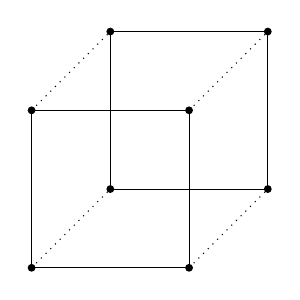
\begin{tikzpicture}[scale=2, every node/.style={circle, inner sep=1pt, fill=black}]
		% Front cube
		\coordinate (A1) at (0,0);
		\coordinate (B1) at (1,0);
		\coordinate (C1) at (1,1);
		\coordinate (D1) at (0,1);
		
		% Back cube
		\coordinate (E1) at (0.5,0.5);
		\coordinate (F1) at (1.5,0.5);
		\coordinate (G1) at (1.5,1.5);
		\coordinate (H1) at (0.5,1.5);
		
		% Draw edges of front cube
		\draw (A1) -- (B1) -- (C1) -- (D1) -- cycle;
		
		% Draw edges of back cube
		\draw (E1) -- (F1) -- (G1) -- (H1) -- cycle;
		
		% Connect corresponding vertices
		\draw[dotted] (A1) -- (E1);
		\draw[dotted] (B1) -- (F1);
		\draw[dotted] (C1) -- (G1);
		\draw[dotted] (D1) -- (H1);
		
		% Draw nodes
		\foreach \p in {A1,B1,C1,D1,E1,F1,G1,H1}
		\node at (\p) {};
	\end{tikzpicture}\hspace{3em}
	\begin{tikzpicture}[scale=2, every node/.style={circle, fill=black, inner sep=1pt}]
		% Define front cube
		\coordinate (A) at (0,0);
		\coordinate (B) at (1,0);
		\coordinate (C) at (1,1);
		\coordinate (D) at (0,1);
		\coordinate (E) at (0.5,0.5);
		\coordinate (F) at (1.5,0.5);
		\coordinate (G) at (1.5,1.5);
		\coordinate (H) at (0.5,1.5);
		
		% Define second set (tesseract projection offset)
		\foreach \p/\q in {A/I, B/J, C/K, D/L, E/M, F/N, G/O, H/P} {
			\coordinate (\q) at ($( \p ) + (.75,.25)$);
		}
		
		% Connect cube edges (front and back)
		\foreach \p/\q in {A/B, B/C, C/D, D/A, E/F, F/G, G/H, H/E,
			A/E, B/F, C/G, D/H,
			I/J, J/K, K/L, L/I, M/N, N/O, O/P, P/M,
			I/M, J/N, K/O, L/P} {
			\draw (\p) -- (\q);
		}
		
		% Connect cube edges (front and back)
		\foreach \p/\q in {
			A/I, B/J, C/K, D/L, E/M, F/N, G/O, H/P} {
			\draw[dotted] (\p) -- (\q);
		}
		
		% Draw nodes
		\foreach \p in {A,B,C,D,E,F,G,H,I,J,K,L,M,N,O,P}
		\node at (\p) {};
	\end{tikzpicture}
\end{center}
	\caption{This figure shows the transition from a single 0-dimensional point to a 4-dimensional tesseract. At each transition, the previous is duplicated (shown in bold lines and points), and the connections from the previous dimension to the new are displayed with dotted lines.}
	\label{fig:cubes-increasing-dimensions}
\end{figure}




Consider the construction of a sphere in multiple dimensions (shown in figure \ref{fig:cubes-increasing-dimensions}). In 0-dimension, there is simply a point. Increasing the dimension by 1 causes the number of points to double. In 1-dimension, this gives 2 points. The number of points doubles with each new dimension, giving $2^d$ points (where $d\in\mathbb{N}$ is the dimension scale). This gives the sequence of points per dimension as 1,2,4,8,16,... When the points in 1-dimension are connected, this makes 1 line segment. The pattern continues as the dimensions increment. 
\begin{align}
	\text{points}(d) = \mathcal{P}_d = 2^d
\end{align}

In 2-dimension, the 2 points from the 1-dimension are duplicated, giving 4 points. The line is also duplicated (in a sense), and new line segments are created to connect the newly created points to the old points. This pattern of line segments also repeats, where the number of new line segments will always be the number of points that existed in the previous dimension (since each point will connect to another new point). Then, the total line segments will be this value summed with the number of line segments from the previous dimension times two (since they are duplicated). Therefore, the number of lines $\ell$ in a dimension is $\mathcal{L}_d = 2\mathcal{L}_{d-1}+2^{d-1}$. This gives the sequence of 0,1,4,12,32,... When these line segments are connected in 2-dimension, they form a square.
\begin{align}
	\text{lines}(d) = \mathcal{L}_d = 2\mathcal{L}_{d-1}+\mathcal{P}_{d-1} = 2\mathcal{L}_{d-1}+2^{d-1}
\end{align}

In 2-dimensions and higher, the geometric element of a square emerges. The square is formed by a combination of 4 lines forming the edges and 4 points forming the corners. In each higher dimension, the squares from the previous dimension are doubled, and then the number of squares increased by the number of lines from the previous dimension. The pattern gives 0,1,6,24,80... When these squares are connected, they form the 3-dimensional cube. The number of squares follows as
\begin{align}
	\text{squares}(d) = \mathcal{S}_d = 2\mathcal{S}_{d-1}+\mathcal{L}_{d-1} = 2\mathcal{S}_{d-1} + 2\mathcal{L}_{d-2}+2^{d-2}
\end{align}

This pattern continues for each new geometric element which emerges from the higher dimensions. Therefore, the number of cubes is
\begin{align}
	\text{cubes}(d) = \mathcal{C}_d = 2\mathcal{C}_{d-1}+\mathcal{S}_{d-1} = 2\mathcal{C}_{d-1} + 2\mathcal{S}_{d-2} + 2\mathcal{L}_{d-3}+2^{d-3}
\end{align}

All of these values for each geometric element are determined based on the values which occur in the dimensions prior. Since the first geometric element (the point) only depends on the dimension, it should be possible to represent the others in terms of only the dimension as well. Writing out the sequences, we can begin to see the patterns outlined in the above sequences emerge:
\begin{equation}
	\renewcommand{\arraystretch}{1.5}
	\begin{tabular}{lc|ccccccccccc}
		&dimension&   0D  &      &   1D   &      &  2D    &      &   3D   &      &  4D    &      &  5D    \\
		\hline
		&points&   1   &      &   2   &      &   4   &      &   8   &      &   16   &      &   32   \\
		&lines&   0   &      &   1   &      &   4   &      &   12   &      &   32   &      &   80   \\
		&squares&   0   &      &   0   &      &   1   &      &   6   &      &   24   &      &   80   \\
		&cubes&    0  &      &   0   &      &   0   &      &   1   &      &   8   &      &   40   \\
		&tesseracts&    0  &      &   0   &      &   0   &      &   0   &      &   1   &      &   10   \\
	\end{tabular}
\end{equation}

A few observations from the above sequences and corresponding formulas are important. First, the row of 1's at the start of the sequence in a diagonal pattern, as well as the continual addition of terms from the previous sequence in each other sequence brings to mind the Pascal Triangle. Recall Pascal's triangle, where each element is determined by the sum of the 2 nearest elements above it. These values give the binomial coefficients of two values $a$ and $b$ as $\binom{a}{b}$.
\begin{equation}
	\renewcommand{\arraystretch}{1.5}
	\begin{tabular}{cccccccccccc}
		&      &      &      &      &      &  1   &      &      &      &      &      \\
		&      &      &      &      &  1   &      &  1   &      &      &      &      \\
		&      &      &      &  1   &      &  2   &      &  1   &      &      &      \\
		&      &      &  1   &      &  3   &      &  3   &      &  1   &      &      \\
		&      &  1   &      &  4   &      &  6   &      &  4   &      &  1   &      \\
		&  1   &      &  5   &      &  10  &      &  10  &      &   5  &      &   1   \\
	\end{tabular}\label{pascals_triangle}
\end{equation}

By writing the pattern such that the values of each is represented as a factored value below it gives the following pattern:
\begin{equation}
	\renewcommand{\arraystretch}{1.5}
	\begin{tabular}{lc|ccccccccccc}
		&dimension&   0D  &      &   1D   &      &  2D    &      &   3D   &      &  4D    &      &  5D    \\
	\hline
	&points&   1   &     &   2    &      &   4    &      &   8  &      &   16   &      &   32   \\
	&      &  (1)  &     &  (1)2  &      &   (1)4 &      & (1)8 &      & (1)16  &      &  (1)32 \\
	&lines&   && 1   &     &   4    &      &   12   &      &   32 &      &   80     \\
	&      &  &&(1)  &     &  (2)2  &      &   (3)4 &      & (4)8 &      &  (5)16   \\
	&squares&  &&&&1   &     &   6    &      &   24   &      &   80   \\
	&      & &&&& (1)  &     &  (3)2  &      &   (6)4 &      & (10)8 \\
	&cubes&   &&&&&& 1   &     &   8    &      &   40    \\
	&      & &&&&&& (1)  &     &  (4)2  &      &  (10)4  \\
	&tesseracts& &&&&&&&&1 &     &   10    \\
	&     &  &&&&&&&&  (1) &     &   (5)2  \\
\end{tabular}
\end{equation}

From this, it's easy to see that the values from Pascal's Triangle emerge as a factor for each value. These values are based on the dimensions $d$ and row $i$. The coefficients matching pascals triangle are then $\binom{d}{i}$. The remaining factor is simply the number of points in each dimension offset by $i$, giving a factor of $2^{d-i}$. Since the rows represent the various geometric sequences, we could assign them to some incremental element starting 0 (representing points), and incrementing. Denote these values of the above table as $\mathbb{G}(d,i)$, where $d$ is the dimension and $i$ represents the geometric element being represented (e.g., $i=0$ would be points, $i=1$ would be lines, $i=2$ would be squares, etc). The values then can be represented as
\begin{align}
	\mathbb{G}(d, i) = \binom{d}{i} 2^{d-i}
\end{align}
This gives the equations and values represented in the following table.
\begin{table}[htbp]
	\centering
	\begin{tabular}{lcccccccc}
		\toprule
		& 0D & 1D & 2D & 3D & 4D & 5D &\dots& \(d\)D \\
		\midrule
		Points     & 1  & 2  & 4  & 8  & 16 & 32 && \(2^d\) \\
		Lines      & 0  & 1  & 4  & 12 & 32 & 80 && \(d \cdot 2^{d-1}\) \\
		Squares    & 0  & 0  & 1  & 6  & 24 & 80 && \(\binom{d}{2} \cdot 2^{d-2}\) \\
		Cubes      & 0  & 0  & 0  & 1  & 8  & 40 && \(\binom{d}{3} \cdot 2^{d-3}\) \\
		Tesseracts & 0  & 0  & 0  & 0  & 1  & 10 && \(\binom{d}{4} \cdot 2^{d-4}\) \\
		\bottomrule
		Sum        & 1  & 3  & 9  & 27  & 81 & 243 && \(3^d\) \\
	\end{tabular}
	\caption{Number of geometric elements in the various dimensions $d$ by constructing cube shapes in higher and lower dimensions. The equations determining the number of each elements is given on the right side. The sum total of the values from each column is also given, as it is a curious result which may be used later.}
	\label{tab:hypercube_elements}
\end{table}

A curious result from table \ref{tab:hypercube_elements}, which is observationally seen by taking the sum of each column is that
\begin{align}
\sum_{d\geq i}^{d}\binom{d}{i}2^{d-i} = 3^d.
\end{align}
Note that this is only valid when $d\geq i$, since the values of $d<i$ are zero in our system, but not zero in the equations representing it.















\subsection{Exploring The Rubik's Cube}

\begin{figure}[h]
	\begin{center}
		\TwoFaceUp
		{W}{W}
		{W}{W}
		\TwoFaceRight
		{R}{R}
		{R}{R}
		\TwoFaceFront
		{G}{G}
		{G}{G}
		\ShowCube{3cm}{0.7}{\DrawTwoCube}
		\begin{minipage}{0.15\linewidth}
		    \centering
		    \scalebox{3}{$\rightarrow$}
		\end{minipage}
		\TwoFaceUp
		{W}{B}
		{W}{B}
		\TwoFaceRight
		{R}{R}
		{R}{R}
		\TwoFaceFront
		{G}{W}
		{G}{W}
		\ShowCube{3cm}{0.7}{\DrawTwoCube}
		
		\vspace{1em}
		
		\RubikFaceUp
		{W}{W}{W}
		{W}{W}{W}
		{W}{W}{W}
		\RubikFaceRight
		{R}{R}{R}
		{R}{R}{R}
		{R}{R}{R}
		\RubikFaceFront
		{G}{G}{G}
		{G}{G}{G}
		{G}{G}{G}
		\ShowCube{3cm}{0.7}{\DrawRubikCube}
		\begin{minipage}{0.15\linewidth}
			\centering
			\scalebox{3}{$\rightarrow$}
		\end{minipage}
		\RubikFaceUp
		{W}{W}{B}
		{W}{W}{B}
		{W}{W}{B}
		\RubikFaceRight
		{R}{R}{R}
		{R}{R}{R}
		{R}{R}{R}
		\RubikFaceFront
		{G}{G}{W}
		{G}{G}{W}
		{G}{G}{W}
		\ShowCube{3cm}{0.7}{\DrawRubikCube}
	
		\caption{Two and three layer Rubik’s cubes shown in solved states (left) and with a single rotation (right).}
		\label{fig:two-cube-and-rubik-cube-simple-turn}
	\end{center}
\end{figure}





